% Created 2023-02-10 Fri 07:31
% Intended LaTeX compiler: pdflatex
\documentclass[presentation,aspectratio=169]{beamer}
\usepackage[utf8]{inputenc}
\usepackage[T1]{fontenc}
\usepackage{graphicx}
\usepackage{grffile}
\usepackage{longtable}
\usepackage{wrapfig}
\usepackage{rotating}
\usepackage[normalem]{ulem}
\usepackage{amsmath}
\usepackage{textcomp}
\usepackage{amssymb}
\usepackage{capt-of}
\usepackage{hyperref}
\usepackage{khpreamble}
\usepackage{amssymb}
\usepgfplotslibrary{groupplots}
\newcommand*{\shift}{\ensuremath{\operatorname{q}}}
\newcommand*{\vecref}[2]{\ensuremath{^#2 \vec{#1}}}
\newcommand*{\pref}[2]{\ensuremath{^#2{#1}}}
\newcommand*{\refsys}[1]{\ensuremath{\{#1\}}}
\newcommand*{\refframe}[4]{%
\draw[->, thick, #4] (0,0) to (#1, 0) node[right]{#2};
\draw[->, thick, #4] (0,0) to (0, #1) node[above]{#3};}
\usetheme{default}
\author{Kjartan Halvorsen}
\date{\today}
\title{Cinemática - Representación de posición y orientación}
\hypersetup{
 pdfauthor={Kjartan Halvorsen},
 pdftitle={Cinemática - Representación de posición y orientación},
 pdfkeywords={},
 pdfsubject={},
 pdfcreator={Emacs 26.3 (Org mode 9.4.6)}, 
 pdflang={English}}
\begin{document}

\maketitle

\section{Intro}
\label{sec:orgd2132b3}
\begin{frame}[label={sec:org0d4980f}]{Brazos robóticos}
\begin{columns}
\begin{column}{0.5\columnwidth}
\begin{center}
 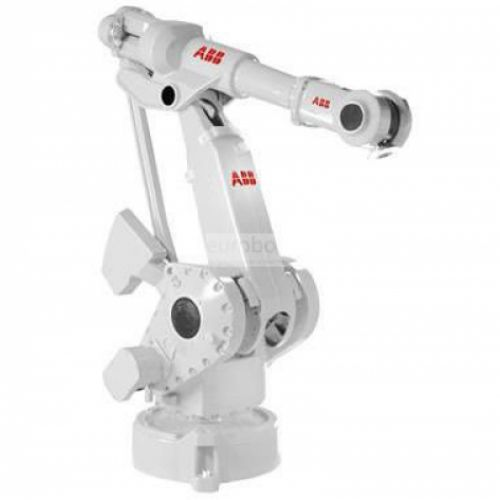
\includegraphics[width=.5\linewidth]{../figures/IRB_4400.jpg}\\
 \tiny Fuente: ABB
\end{center}

\pause

\begin{center}
 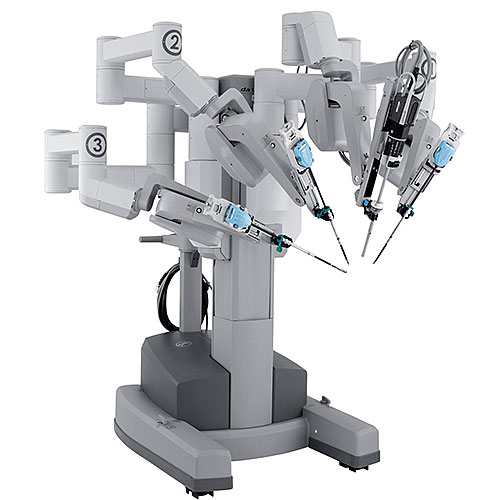
\includegraphics[width=.5\linewidth]{../figures/davinci.jpg}\\
\tiny Intuitive
\end{center}

\pause
\end{column}


\begin{column}{0.5\columnwidth}
\begin{center}
 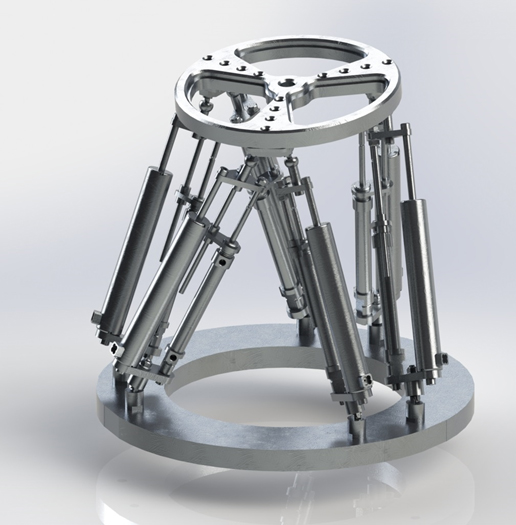
\includegraphics[width=.5\linewidth]{../figures/stewart.jpg}\\
 \tiny Fuente: Amir Yazdani

\end{center}
\pause

\begin{center}
 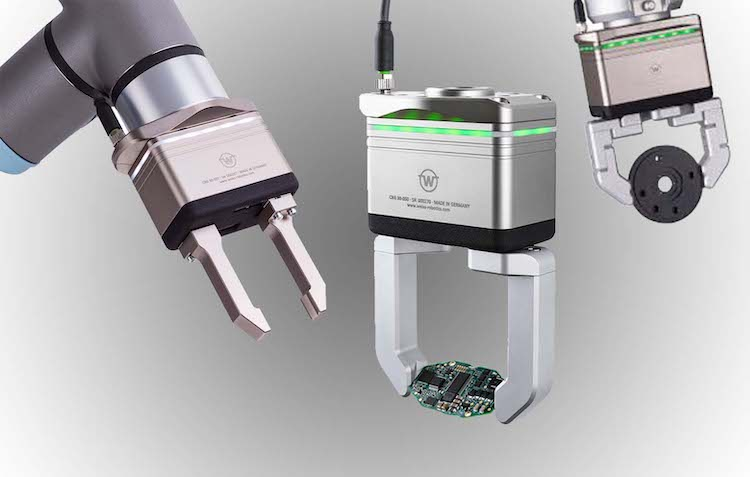
\includegraphics[width=.7\linewidth]{../figures/gripper.jpg}\\
 \tiny Fuente: Robotics \& Automation news
\end{center}
\end{column}
\end{columns}
\end{frame}



\begin{frame}[label={sec:orga16ae4f}]{Definiciones}
\begin{center}
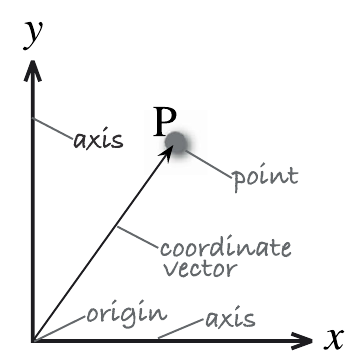
\includegraphics[height=0.5\textheight]{../figures/Corke-fig2.1.a.png}

\footnotesize Peter Corke \emph{Robotics, vision and control}
\end{center}
\end{frame}


\begin{frame}[label={sec:org0438fc8}]{Uso de sistemas de referencia en robótica}
\begin{center}
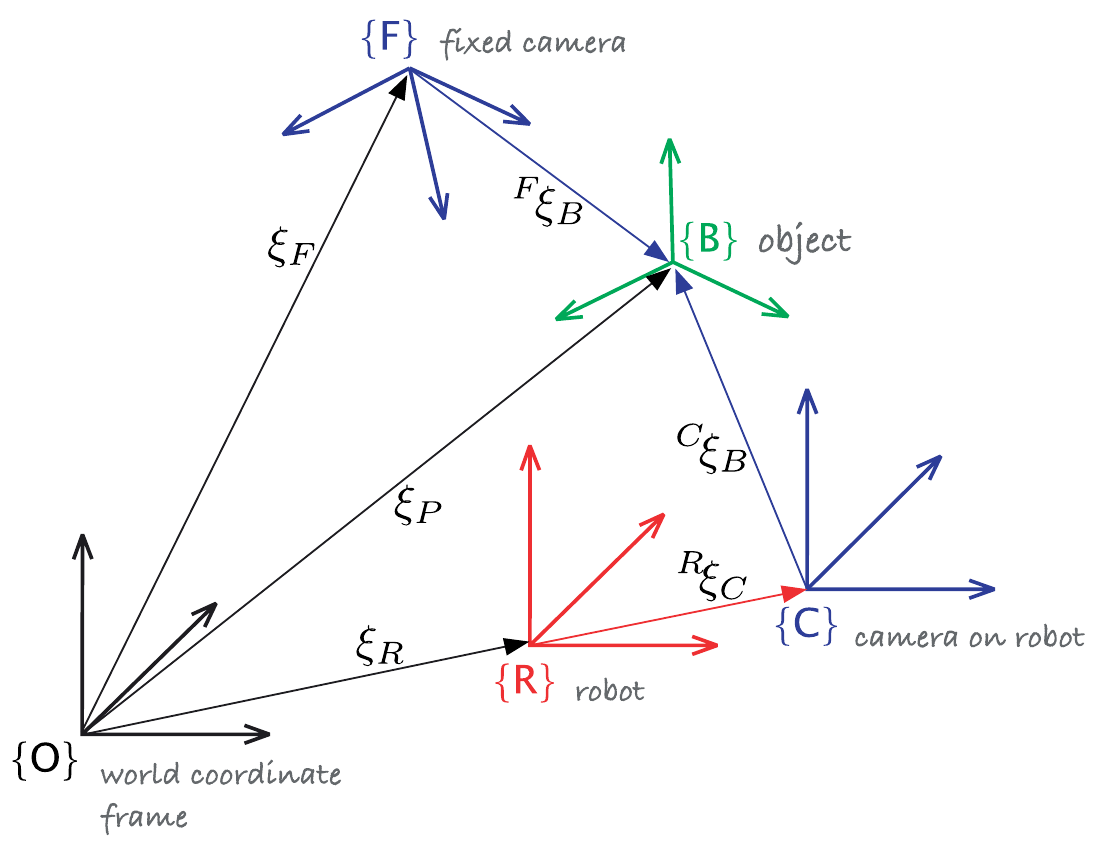
\includegraphics[height=0.5\textheight]{../figures/Corke-fig2.4.png}

\footnotesize Peter Corke \emph{Robotics, vision and control}
\end{center}
\end{frame}
\end{document}